\documentclass[12pt]{article}
\usepackage{graphicx}
\usepackage{subcaption}
\usepackage{mwe}
\usepackage[]{mcode}
%\usepackage{lingmacros}
%\usepackage{tree-dvips}
%\usepackage{blindtext}
%\usepackage[utf8]{inputenc}

\begin{document}

\title{CMSC 426 - HW1}
\author{Gudjon Einar Magnusson}

\maketitle

\section{Blobs}

\subsection{My Region Props}

\subsubsection{Area}
\begin{minipage}{\linewidth}
\begin{lstlisting}
    %% Count number of pixesl in blob
    stats(count).Area = sum(sum(CurrBlob));
\end{lstlisting}
\end{minipage}

\subsubsection{Centroid}
\begin{minipage}{\linewidth}
\begin{lstlisting}
    %% Find index of non-zero elements
    [r, c] = find(CurrBlob);
    n = size(r, 1);
    %% Compute avarege of all non-zero pixel coordinates
    stats(count).Centroid = [sum(c)/n, sum(r)/n];
\end{lstlisting}
\end{minipage}

\subsubsection{Bounding Box}
\begin{minipage}{\linewidth}
\begin{lstlisting}
    %% Find index of non-zero elements
    [r, c] = find(CurrBlob);
    %% Find bounds and add padding
    maxCol = max(c) + 0.5;
    minCol = min(c) - 0.5;
    maxRow = max(r) + 0.5;
    minRow = min(r) - 0.5;
    stats(count).BoundingBox = [minCol, minRow, maxCol-minCol, maxRow-minRow];
\end{lstlisting}
\end{minipage}

\section{Gabor Filters}

\section{Resizing}

Figure\ref{fig_scale} shows the sample image scaled up and down. The effect may be hard to see on paper, but I promise its amazing.

\begin{figure}
    \begin{subfigure}[t]{.49\textwidth}
        \centering
        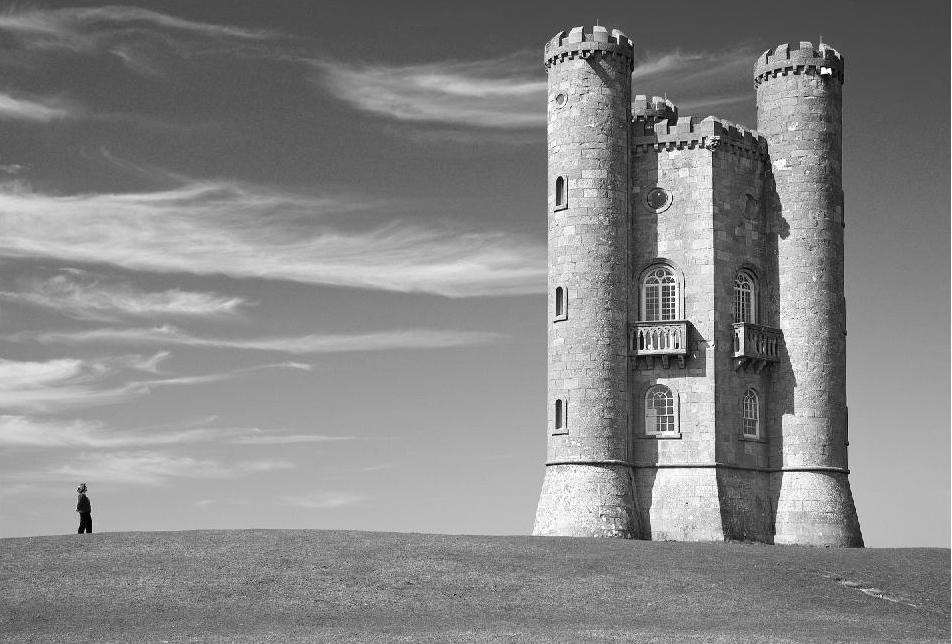
\includegraphics[width=\linewidth]{resize_double}
        \caption{Scaled up 100\%}
    \end{subfigure}\hfill
    \begin{subfigure}[t]{.49\textwidth}
        \centering
        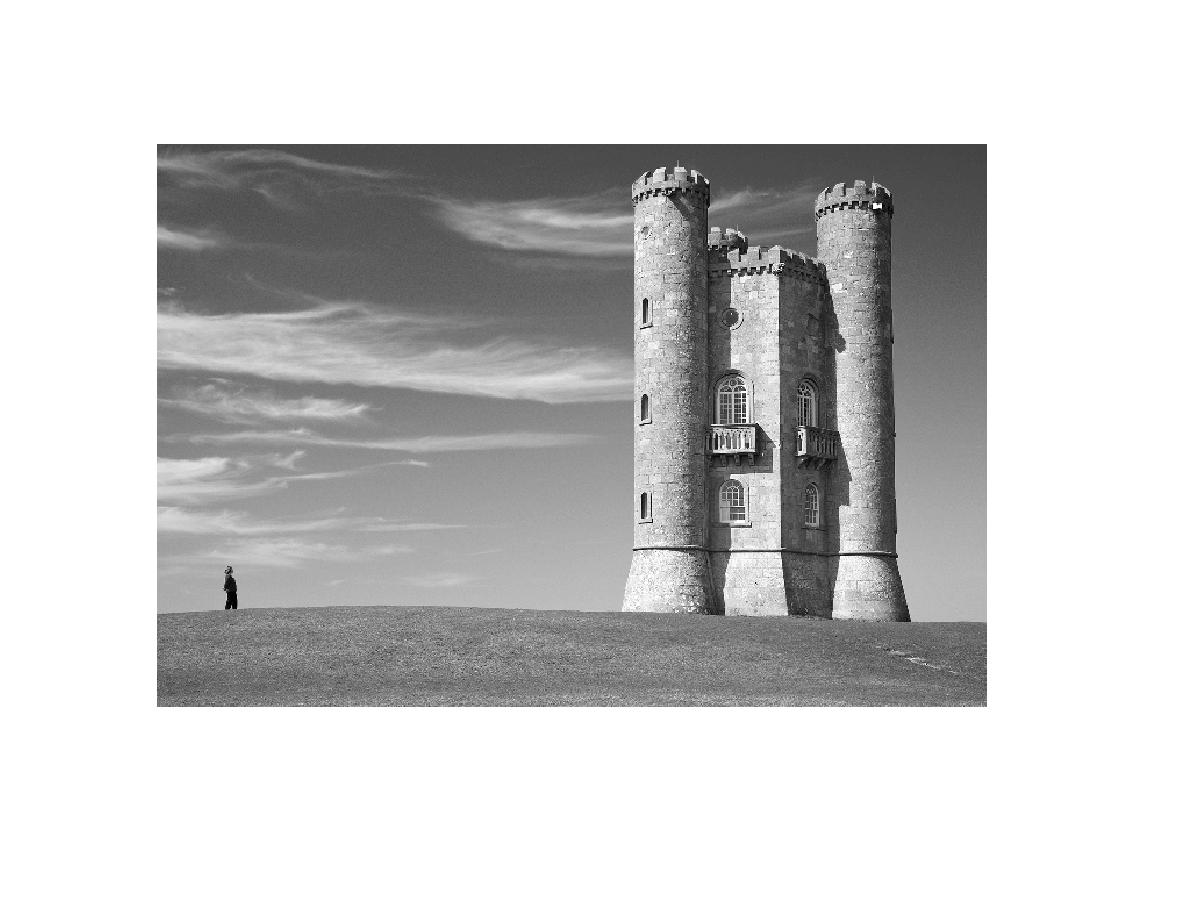
\includegraphics[width=\linewidth]{resize_half}
        \caption{Scaled down 50\%}
    \end{subfigure}
    \label{fig_scale}
\end{figure}


\section{Anisotropic Filter}

$K$ effectively defines how much contrast is needed to count as an edge. I high value of $K$ means causes a pixel to more likely to be affected by a neighboring pixel that is different, edges are more likely to blur. A low value of $K$ means that more things are counted as edges, lines that there previously not visible may be sharpened.

$\lambda$ defines how much change is allowed per iteration. A low value means that more iterations are needed but the result is smoother. A high value means that each iteration can make big changes and that can cause noise and weird patterns. 

\section{Eigen Faces}

A bug in my implementation causes the recognition rate to be very low, only 2.5\%. In my case 13 seems to be a good value for $k$. Anything above 13 gives no improvement but below 13 the recognition rate quickly drops.


\section{Seam Carving}

For the seam carving algorithm I use an energy function that is simply the gradient of each pixel. The gradient is calculated by applying the \textit{imgradient} function on a grayscale version of the image.

Unfortunately my seam carving implementation is not very optimized, so to save some time reduced the size of the sample image by 50\%.
In figure \ref{fig_carve} you can see the result of carving 50 horizontal and 100 vertical seams from the sample image. Overall the results are descent but unfortunately the person in the picture is cut in half, this is the most notable flaw. 


\begin{figure}
    \begin{subfigure}[t]{.49\textwidth}
        \centering
        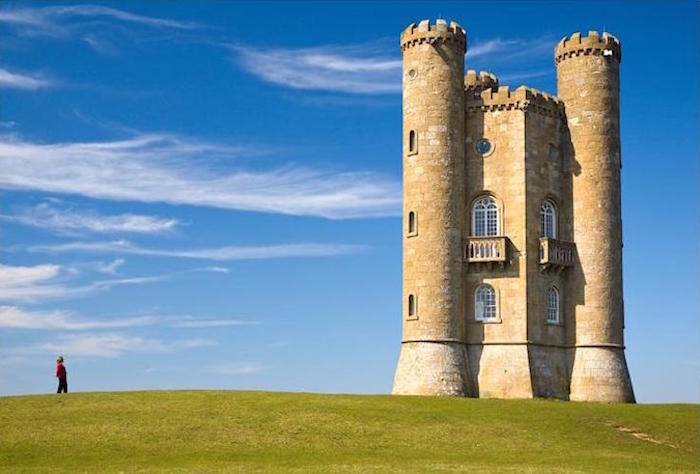
\includegraphics[width=\linewidth]{carving_original}
    \end{subfigure}\hfill
    \begin{subfigure}[t]{.47\textwidth}
        \centering
        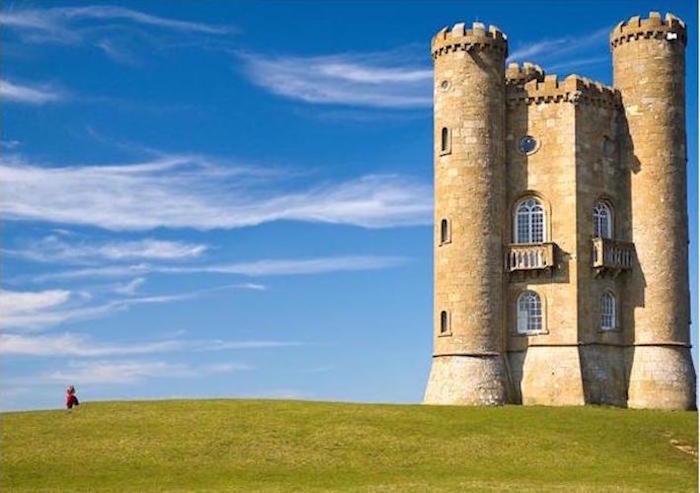
\includegraphics[width=\linewidth]{carving_50_100}
    \end{subfigure}
    \caption{Before and after seam carving}
    \label{fig_carve}
\end{figure}

\end{document}